\documentclass[]{jarticle}          % 一段組
%\documentclass[twocolumn]{jarticle} % 二段組

\textwidth 180mm
\textheight 255mm
\oddsidemargin -12mm
\topmargin -15mm
\columnsep 10mm

%\vspace{0.5cm} % 一段組の場合はコメントアウトした方が体裁がよいx
%] % 一段組の場合はコメントアウトする

\usepackage{styles/labheadings}
\usepackage[dvipdfmx]{graphicx,color}
\usepackage{amsmath,amssymb}
\usepackage{url}
% 追加
\usepackage{listings,jvlisting}
\usepackage[hang,small,bf]{caption}
\usepackage[subrefformat=parens]{subcaption}
\usepackage{bm}
\captionsetup{compatibility=false}

\newcommand{\aU}{\mbox{\boldmath $a$}}
\newcommand{\bU}{\mbox{\boldmath $b$}}
\newcommand{\cU}{\mbox{\boldmath $c$}}
\newcommand{\dU}{\mbox{\boldmath $d$}}
\newcommand{\eU}{\mbox{\boldmath $e$}}
\newcommand{\fU}{\mbox{\boldmath $f$}}
\newcommand{\gU}{\mbox{\boldmath $g$}}
\newcommand{\hU}{\mbox{\boldmath $h$}}
\newcommand{\iU}{\mbox{\boldmath $i$}}
\newcommand{\jU}{\mbox{\boldmath $j$}}
\newcommand{\kU}{\mbox{\boldmath $k$}}
\newcommand{\lU}{\mbox{\boldmath $l$}}
\newcommand{\mU}{\mbox{\boldmath $m$}}
\newcommand{\nU}{\mbox{\boldmath $n$}}
\newcommand{\oU}{\mbox{\boldmath $o$}}
\newcommand{\pU}{\mbox{\boldmath $p$}}
\newcommand{\qU}{\mbox{\boldmath $q$}}
\newcommand{\rU}{\mbox{\boldmath $r$}}
\newcommand{\sU}{\mbox{\boldmath $s$}}
\newcommand{\tU}{\mbox{\boldmath $t$}}
\newcommand{\uU}{\mbox{\boldmath $u$}}
\newcommand{\vU}{\mbox{\boldmath $v$}}
\newcommand{\wU}{\mbox{\boldmath $w$}}
\newcommand{\xU}{\mbox{\boldmath $x$}}
\newcommand{\yU}{\mbox{\boldmath $y$}}
\newcommand{\zU}{\mbox{\boldmath $z$}}
\newcommand{\AU}{\mbox{\boldmath $A$}}
\newcommand{\BU}{\mbox{\boldmath $B$}}
\newcommand{\CU}{\mbox{\boldmath $C$}}
\newcommand{\DU}{\mbox{\boldmath $D$}}
\newcommand{\EU}{\mbox{\boldmath $E$}}
\newcommand{\FU}{\mbox{\boldmath $F$}}
\newcommand{\GU}{\mbox{\boldmath $G$}}
\newcommand{\HU}{\mbox{\boldmath $H$}}
\newcommand{\IU}{\mbox{\boldmath $I$}}
\newcommand{\JU}{\mbox{\boldmath $J$}}
\newcommand{\KU}{\mbox{\boldmath $K$}}
\newcommand{\LU}{\mbox{\boldmath $L$}}
\newcommand{\MU}{\mbox{\boldmath $M$}}
\newcommand{\NU}{\mbox{\boldmath $N$}}
\newcommand{\OU}{\mbox{\boldmath $O$}}
\newcommand{\PU}{\mbox{\boldmath $P$}}
\newcommand{\QU}{\mbox{\boldmath $Q$}}
\newcommand{\RU}{\mbox{\boldmath $R$}}
\newcommand{\SU}{\mbox{\boldmath $S$}}
\newcommand{\TU}{\mbox{\boldmath $T$}}
\newcommand{\UU}{\mbox{\boldmath $U$}}
\newcommand{\VU}{\mbox{\boldmath $V$}}
\newcommand{\WU}{\mbox{\boldmath $W$}}
\newcommand{\XU}{\mbox{\boldmath $X$}}
\newcommand{\YU}{\mbox{\boldmath $Y$}}
\newcommand{\ZU}{\mbox{\boldmath $Z$}}
\newcommand{\epU}{\mbox{\boldmath $\epsilon$}}
\newcommand{\taU}{\mbox{\boldmath $\tau$}}
\newcommand{\etU}{\mbox{\boldmath $\eta$}}
\newcommand{\xiU}{\mbox{\boldmath $\xi$}}
\newcommand{\wwU}{\mbox{\boldmath $\omega$}}
\newcommand{\WwU}{\mbox{\boldmath $\Omega$}}
\newcommand{\lmU}{\mbox{\boldmath $\lambda$}}
\newcommand{\LmU}{\mbox{\boldmath $\Lambda$}}
\newcommand{\PiU}{\mbox{\boldmath $\Pi$}}
\newcommand{\SgU}{\mbox{\boldmath $\Sigma$}}
\newcommand{\thU}{\mbox{\boldmath $\theta$}}
\newcommand{\ThU}{\mbox{\boldmath $\Theta$}}
\newcommand{\roU}{\mbox{\boldmath $\rho$}}
\newcommand{\nuU}{\mbox{\boldmath $\nu$}}
\newcommand{\ones}{{\bf 1}}
\newcommand{\zr}{{\bf 0}}
\newcommand{\eq}{\begin{equation}}
\newcommand{\en}{\end{equation}}
\newcommand{\eqa}{\begin{eqnarray}}
\newcommand{\ena}{\end{eqnarray}}
\newcommand{\xx}{\makebox[1cm]{}}
\newcommand{\xm}{\makebox[0.5cm]{}}
\newcommand{\x}{\makebox[0.2cm]{}}
\newcommand{\tr}{{\rm tr}}
\newcommand{\sgn}{{\rm sgn}}
\newcommand{\ad}{{\rm ad}}

\newcommand{\rank}{{\rm rank}}
\newcommand{\diag}{{\rm diag}}
\newcommand{\lbr}{\left(\begin{array}}
\newcommand{\rbr}{\end{array}\right)}
\newcommand{\Proof}{\noindent{\em Proof\/}}
\newcommand{\Solution}{\noindent{\em Solution}}
\newcommand{\Derivation}{\noindent{\em Derivation}}
\newcommand{\msp}{\vspace*{\medskipamount}\\}
\newcommand{\qed}{\hspace*{\fill}$\Box$}
\newcommand{\aX}{{\bf a}}
\newcommand{\bX}{{\bf b}}
\newcommand{\cX}{{\bf c}}
\newcommand{\dX}{{\bf d}}
\newcommand{\eX}{{\bf e}}
\newcommand{\fX}{{\bf f}}
\newcommand{\gX}{{\bf g}}
\newcommand{\hX}{{\bf h}}
\newcommand{\iX}{{\bf i}}
\newcommand{\jX}{{\bf j}}
\newcommand{\kX}{{\bf k}}
\newcommand{\lX}{{\bf l}}
\newcommand{\mX}{{\bf m}}
\newcommand{\nX}{{\bf n}}
\newcommand{\oX}{{\bf o}}
\newcommand{\pX}{{\bf p}}
\newcommand{\qX}{{\bf q}}
\newcommand{\rX}{{\bf r}}
\newcommand{\sX}{{\bf s}}
\newcommand{\tX}{{\bf t}}
\newcommand{\uX}{{\bf u}}
\newcommand{\vX}{{\bf v}}
\newcommand{\wX}{{\bf w}}
\newcommand{\xX}{{\bf x}}
\newcommand{\yX}{{\bf y}}
\newcommand{\zX}{{\bf z}}
\newcommand{\AX}{{\bf A}}
\newcommand{\BX}{{\bf B}}
\newcommand{\CX}{{\bf C}}
\newcommand{\DX}{{\bf D}}
\newcommand{\EX}{{\bf E}}
\newcommand{\FX}{{\bf F}}
\newcommand{\GX}{{\bf G}}
\newcommand{\HX}{{\bf H}}
\newcommand{\IX}{{\bf I}}
\newcommand{\JX}{{\bf J}}
\newcommand{\KX}{{\bf K}}
\newcommand{\LX}{{\bf L}}
\newcommand{\MX}{{\bf M}}
\newcommand{\NX}{{\bf N}}
\newcommand{\OX}{{\bf O}}
\newcommand{\PX}{{\bf P}}
\newcommand{\QX}{{\bf Q}}
\newcommand{\RX}{{\bf R}}
\newcommand{\SX}{{\bf S}}
\newcommand{\TX}{{\bf T}}
\newcommand{\UX}{{\bf U}}
\newcommand{\VX}{{\bf V}}
\newcommand{\WX}{{\bf W}}
\newcommand{\XX}{{\bf X}}
\newcommand{\YX}{{\bf Y}}
\newcommand{\ZX}{{\bf Z}}

% report.texと同じディレクトリにnumerical_definition.texを入れておけば上の書き方でもいいはずです

\usepackage[
  dvipdfm,
  bookmarks=true,
  bookmarksnumbered=true,
  colorlinks=true]{hyperref}
\AtBeginDvi{\special{pdf:tounicode EUC-UCS2}}

%ここからソースコードの表示に関する設定
\lstset{
  basicstyle={\ttfamily},
  identifierstyle={\small},
  commentstyle={\smallitshape},
  keywordstyle={\small\bfseries},
  ndkeywordstyle={\small},
  stringstyle={\small\ttfamily},
  frame={tb},
  breaklines=true,
  columns=[l]{fullflexible},
  numbers=left,
  xrightmargin=0zw,
  xleftmargin=3zw,
  numberstyle={\scriptsize},
  stepnumber=1,
  numbersep=1zw,
  lineskip=-0.5ex
}
%ここまでソースコードの表示に関する設定

\pagestyle{labheadings}
\headerleft{進捗報告}   % ヘッダの左側のタイトル
\headerright{2023年12月5日}  % ヘッダの右側のタイトル

\begin{document}

%\twocolumn % 一段組の場合はコメントアウトする

\vspace*{2ex}
\begin{center}
 {\Large \bf マスクをした顔画像からの安定したカメラ姿勢推定と、マスクなし顔画像の再現
 }\\ % タイトル
 \vspace*{5mm}
 {\large B4 田川幸汰}% 発表者名
\end{center}

%\vspace{0.5cm} % 一段組の場合はコメントアウトした方が体裁がよいx
%] % 一段組の場合はコメントアウトする

%新しく作成したコマンド
% \newcommand{\reffig}[1]{\hyperref[#1]{図\ref{#1}}}
% \newcommand{\refeq}[1]{\hyperref[#1]{式(\ref{#1})}}
% \newcommand{\reftab}[1]{\hyperref[#1]{表\ref{#1}}}
% \newcommand{\refsec}[1]{\hyperref[#1]{\ref{#1}章}}
% \newcommand{\refsubsec}[1]{\hyperref[#1]{\ref{#1}節}}

% 数式
%\begin{equation}
%  数式記述  
%  \label{ラベル名}
%\end{equation}

% 図
% \begin{figure}[!ht]
%   \begin{center}
%     \includegraphics[scale=0.5]{figures/画像ファイル名}
%     \caption{キャプション名}
%     \label{ラベル名}
%   \end{center}
% \end{figure}

% リスト
% \begin{enumerate or itemize}
%   \item 
% \end{enumerate or itemize}

\section{推定結果の誤差の評価}
マスク着用時と非着用時を比較して、カメラ姿勢推定に用いる顔の二次元座標の誤差について評価する。

\subsection{評価方法}
マスク着用時とマスク非着用時で、同一の位置及び姿勢で顔認識を行い取得したランドマークの二次元座標の差を求めることで、顔認識のずれについて評価する。マスク非着用時の二次元座標を
真値として、マスク着用時の二次元座標との差を誤差とする。
以下に評価方法を示す。
\begin{itemize}
  \item 座標の計測を行うランドマークは、顔上部の計151点
  \item 計測を行う顔の角度は、X軸周りの回転角が25°、40°、-25°、-40°
  \item 顔の角度は、マスクを着用していない状態で計算
  \item 顔の角度が正の時は顔の左側の座標のずれを計測、負の時は顔の右側の座標のずれを計測、
  \item 結果は、小数点以下四桁で切り捨て
\end{itemize}

\subsection{結果}
マスク非着用時と非着用時の座標のずれが最大、及び最小になったランドマークの二次元座標の差を\hyperref[n321]{表\ref{n321}}に示す。

\begin{table}[ht!]
  \begin{center}
    \begin{tabular}{lrrrr}
      & 25° & 40° & -25° & 40° \\
      x座標のずれ最小 &  &  &  &  \\
      x座標のずれ最大 &  &  &  &  \\
      y座標のずれ最小 &  &  &  &  \\
      y座標のずれ最大 &  &  &  & 
    \end{tabular}
    \caption{ずれが最大/最小の誤差の値}
    \label{n321}
  \end{center}
\end{table}



また、ずれの大きさを座標の色で表したものを\hyperref[n322]{図\ref{n322}}、
\hyperref[n323]{図\ref{n323}}、\hyperref[n324]{図\ref{n324}}に示す。赤色が濃いと誤差が小さく、赤色が薄いと誤差が大きいことを表す。

\begin{figure}[!ht]
  \begin{tabular}{cc}
    \begin{minipage}[t]{0.45\hsize}
      \centering
      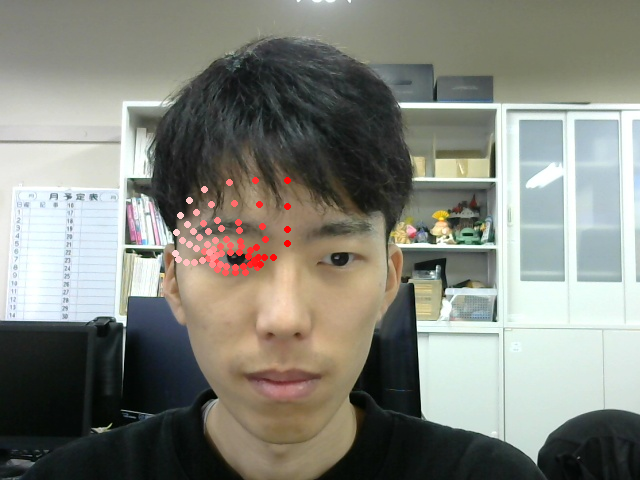
\includegraphics[keepaspectratio, scale=0.3]{figures/error_result/rank_lx_1.png}
      \caption{$X$座標の誤差(顔左部)}
    \end{minipage} &
    \begin{minipage}[t]{0.45\hsize}
      \centering
      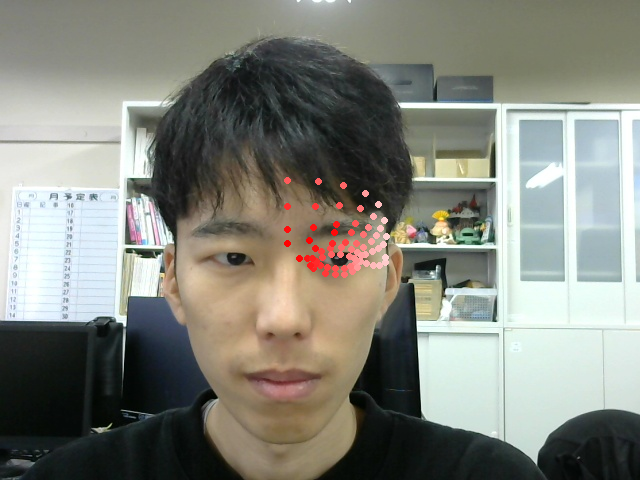
\includegraphics[keepaspectratio, scale=0.3]{figures/error_result/rank_rx_1.png}
      \caption{$X$座標の誤差(顔右部)}
    \end{minipage}
  \end{tabular}
  \caption{マスク着用前後の$X$座標の誤差}
  \label{n322}
\end{figure}

\begin{figure}[!ht]
  \begin{tabular}{cc}
    \begin{minipage}[t]{0.45\hsize}
      \centering
      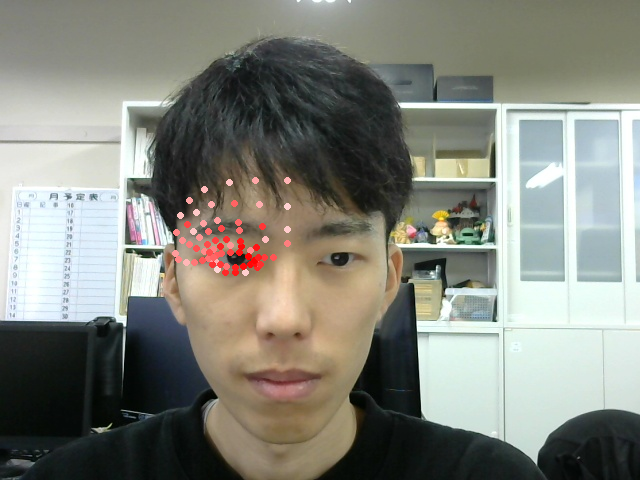
\includegraphics[keepaspectratio, scale=0.3]{figures/error_result/rank_ly_1.png}
      \caption{$Y$座標の誤差(顔左部)}
    \end{minipage} &
    \begin{minipage}[t]{0.45\hsize}
      \centering
      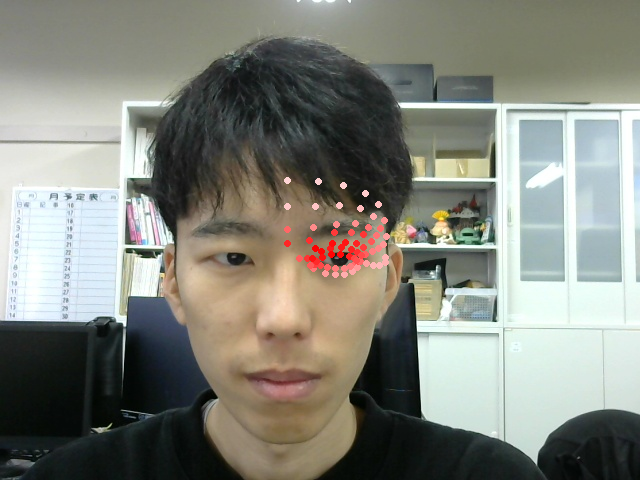
\includegraphics[keepaspectratio, scale=0.3]{figures/error_result/rank_ry_1.png}
      \caption{$Y$座標の誤差(顔右部)}
    \end{minipage}
  \end{tabular}
  \caption{マスク着用前後の$Y$座標の誤差}
  \label{n323}
\end{figure}

\begin{figure}[!ht]
  \begin{tabular}{cc}
    \begin{minipage}[t]{0.45\hsize}
      \centering
      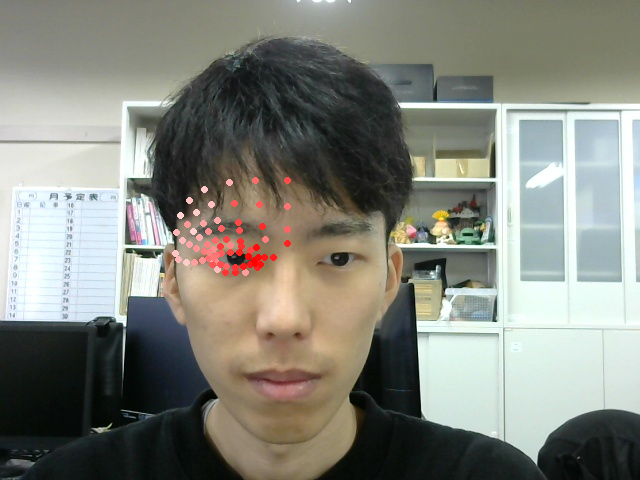
\includegraphics[keepaspectratio, scale=0.3]{figures/error_result/rank_l_1.png}
      \caption{X,Y座標の誤差の合計(顔左部)}
    \end{minipage} &
    \begin{minipage}[t]{0.45\hsize}
      \centering
      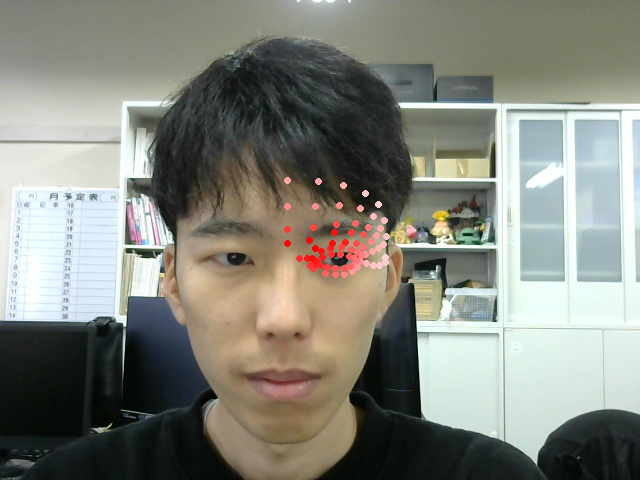
\includegraphics[keepaspectratio, scale=0.3]{figures/error_result/rank_r_1.png}
      \caption{X,Y座標の誤差の合計(顔左部)}
    \end{minipage}
  \end{tabular}
  \caption{マスク着用前後の$X,Y$座標の誤差の合計}
  \label{n324}
\end{figure}

$X$座標については目の周辺部や顔の中心部分が、マスク着用前後の座標のずれが小さく、顔の左端、右端は座標のずれがが大きくなっていることがわかる。
また、$Y$座標については目の周辺部がずれが小さく、顔の上端はずれが大きくなっていることがわかる。
さらに、$X$座標と$Y$座標の誤差を足した値については、目の周辺部に近づくにつれずれが小さくなっていると考えられる。

\subsection{考察}
結果から、目の周辺や顔の中心部のランドマークの二次元座標は、マスク着用前後で比較的安定して推定することができていると判断する。
以降の章で、これらの二次元座標のみをカメラ姿勢推定の対応点として利用した場合と、そうでない場合とで推定結果を比較し、
カメラ姿勢推定の安定性が向上したかについて検証する。


\section{システムの実行とカメラ位置姿勢推定の評価}
マスクを着用した顔画像からマスクなし顔画像を再現する。
また、マスク着用時と非着用時を比較して、カメラ姿勢推定の結果がどう変化したか評価する。
\subsection{評価方法}
マスク着用時とマスク非着用時で、同一の位置及び姿勢で顔認識を行い、取得したランドマークの二次元座標を用いてカメラ姿勢推定を行う。
推定結果を基に、マスク着用時は三次元モデルを張り合わせマスクなし顔画像を再現する。
\begin{itemize}
  \item 入力するマスク着用画像は、\hyperref[n431]{図\ref{n431}}に示す4枚
  \item 検証を行う顔の角度は、X軸周りの回転角が25°、40°、-25°、-40°
  \item 顔の角度は、マスクを着用していない状態で計算
  \item 座標の計測を行うランドマークは、顔上部の計x点
  \item 結果は、小数点以下四桁で切り捨て
\end{itemize}

\begin{figure}[!ht]
  \begin{tabular}{cccc}
    \begin{minipage}[t]{0.25\hsize}
      \centering
      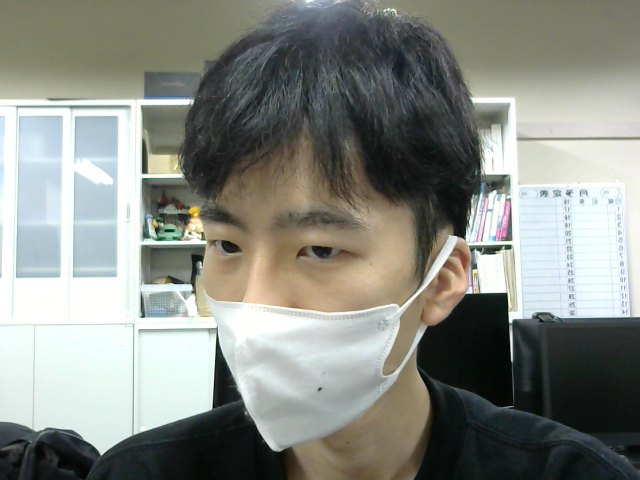
\includegraphics[keepaspectratio, scale=0.2]{figures/result/0mask.png}
      \caption{25°}
    \end{minipage} &
    \begin{minipage}[t]{0.25\hsize}
      \centering
      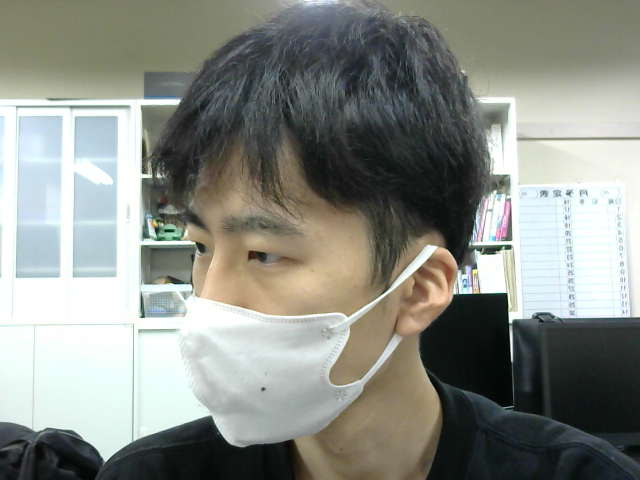
\includegraphics[keepaspectratio, scale=0.2]{figures/result/3mask.png}
      \caption{40°}
    \end{minipage}
    \begin{minipage}[t]{0.25\hsize}
      \centering
      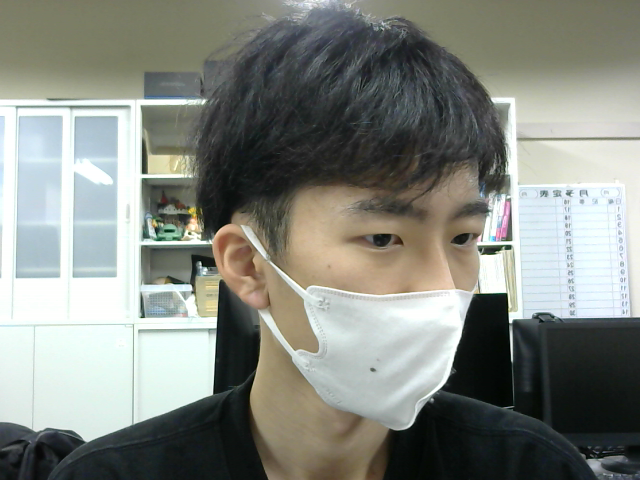
\includegraphics[keepaspectratio, scale=0.2]{figures/result/4mask.png}
      \caption{-25°}
    \end{minipage}
    \begin{minipage}[t]{0.25\hsize}
      \centering
      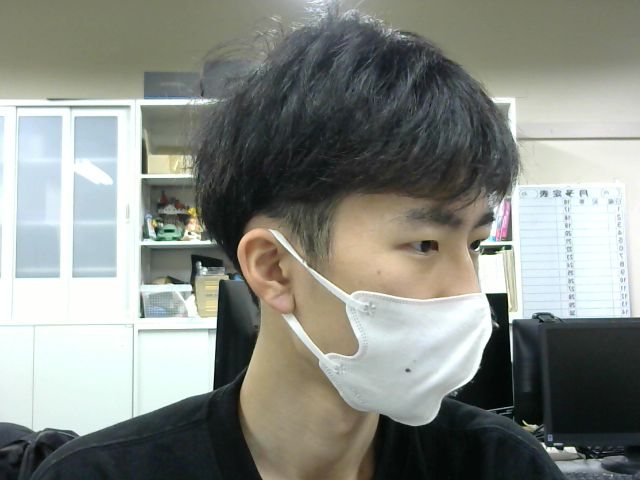
\includegraphics[keepaspectratio, scale=0.2]{figures/result/7mask.png}
      \caption{40°}
    \end{minipage}
  \end{tabular}
  \caption{入力画像}
  \label{n431}
\end{figure}

\subsection{マスクなし画像の再現結果}
再現したマスク非着用画像を\hyperref[n431]{図\ref{n432}}に示す。
\begin{figure}[!ht]
  \begin{tabular}{cccc}
    \begin{minipage}[t]{0.25\hsize}
      \centering
      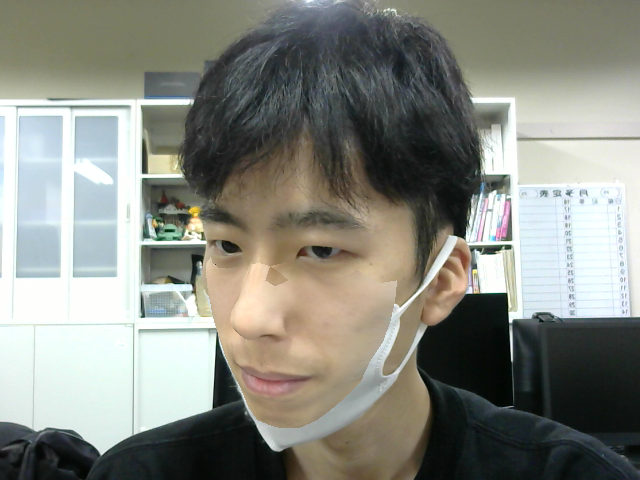
\includegraphics[keepaspectratio, scale=0.2]{figures/result/0mask/image_20231202-2.png}
      \caption{25°}
    \end{minipage} &
    \begin{minipage}[t]{0.25\hsize}
      \centering
      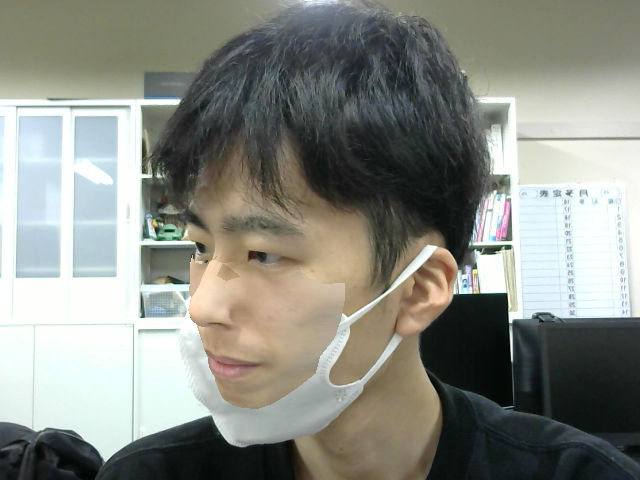
\includegraphics[keepaspectratio, scale=0.2]{figures/result/3mask/image_20231202-2.png}
      \caption{40°}
    \end{minipage}
    \begin{minipage}[t]{0.25\hsize}
      \centering
      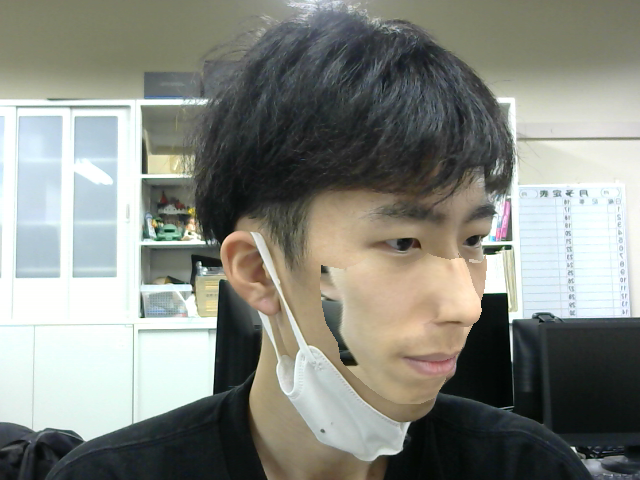
\includegraphics[keepaspectratio, scale=0.2]{figures/result/4mask/image_20231202-2.png}
      \caption{-25°}
    \end{minipage}
    \begin{minipage}[t]{0.25\hsize}
      \centering
      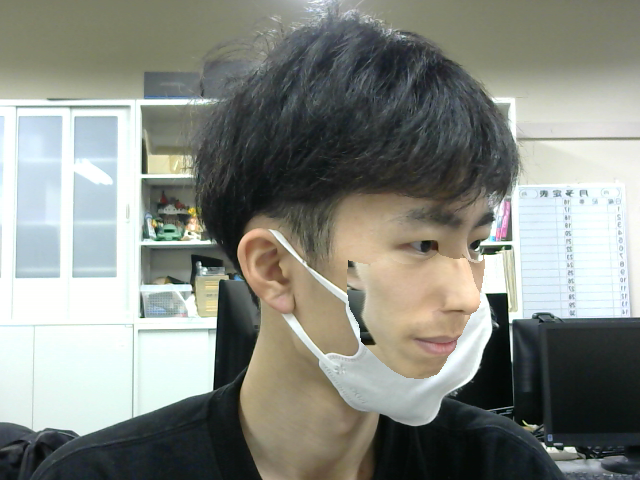
\includegraphics[keepaspectratio, scale=0.2]{figures/result/7mask/image_20231202-2.png}
      \caption{40°}
    \end{minipage}
  \end{tabular}
  \caption{再現したマスク非着用画像}
  \label{n432}
\end{figure}

顔の$X$軸周りの回転角が25°、-25°の場合はマスク非着用画像が十分再現できているとわかる。
顔の$X$軸周りの回転角が40°、-40°の場合についても再現できているが、三次元モデルが少し小さく表示されているように感じる。
また、システムの実装の様子についても、顔の$X$軸周りの回転角が40°以下の場合は安定してマスク非着用画像を再現することができている。
しかし、回転角が40°を超えてしまうと、顔認識が正常に動作せず、再現を行うことが難しくなってしまう。また、顔の$Y$軸周りの回転角については15°を超えてしまうと、
こちらも顔認識が正常に動作せず、再現を行うことが難しくなってしまう。

\section{マスク着用時のカメラ位置姿勢推定の安定性の向上}
カメラ位置姿勢推定に用いるランドマークを、マスク着用前後で座標が比較的安定して推定することができているランドマークのみ用いることで、
カメラ位置姿勢推定の安定性が向上したかどうか評価する。

\subsection{評価方法}
マスク着用時とマスク非着用時で、同一の位置及び姿勢で顔認識を行い、取得したランドマークの二次元座標を用いてカメラ姿勢推定を行う。
推定結果を基に、マスク着用時は三次元モデルを張り合わせマスクなし顔画像を再現する。
\begin{itemize}
  \item 入力するマスク着用画像は、\hyperref[n431]{図\ref{n431}}に示す4枚
  \item 検証を行う顔の角度は、$X$軸周りの回転角が40°
  \item 顔の角度は、マスクを着用していない状態で計算
  \item 使用する対応点は、\hyperref[n441]{図\ref{n441}}、\hyperref[n442]{図\ref{n442}}、\hyperref[n443]{図\ref{n443}}の全6通り
  \item 色付きの対応点は、前章の検証でマスク着用前後で安定していると判断した点を使用
  \item \hyperref[n442]{図\ref{n442}}の対応点は顔の$X$軸周りの回転角が正の時、\hyperref[n443]{図\ref{n443}}は負の時のみ使用
  \item 結果は、小数点以下四桁で切り捨て
\end{itemize}

\begin{figure}[!ht]
  \begin{tabular}{ccc}
    \begin{minipage}[t]{0.33\hsize}
      \centering
      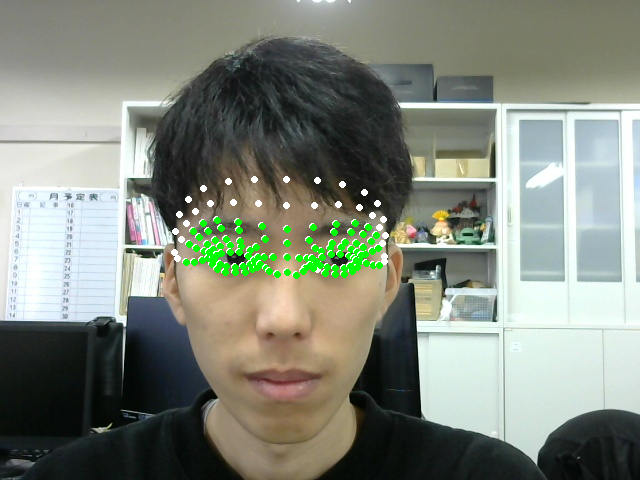
\includegraphics[scale=0.2]{figures/result/landmark_all.png}
      \caption{使用する対応点(顔上部全体)}
      \label{n441}
    \end{minipage} &
    \begin{minipage}[t]{0.33\hsize}
      \centering
      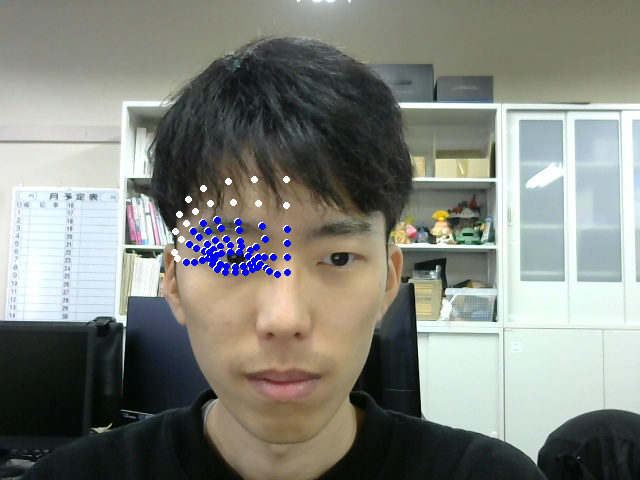
\includegraphics[scale=0.2]{figures/result/landmark_left.png}
      \caption{使用する対応点(顔左上部)}
      \label{n442}
    \end{minipage}
    \begin{minipage}[t]{0.33\hsize}
      \centering
      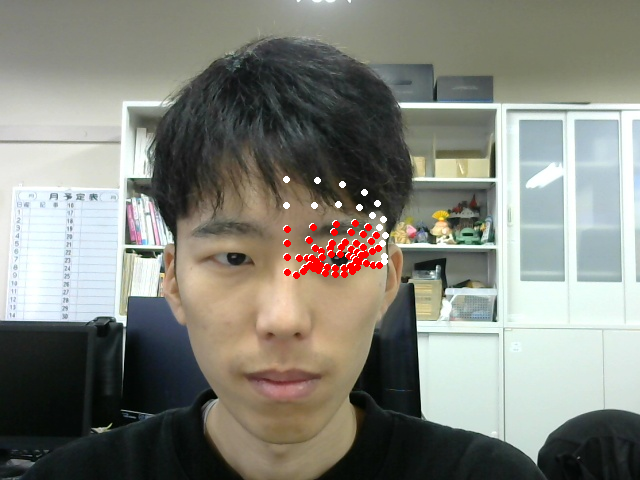
\includegraphics[scale=0.2]{figures/result/landmark_right.png}
      \caption{使用する対応点(顔右上部)}
      \label{n443}
    \end{minipage}
  \end{tabular}
\end{figure}

\subsection{マスクなし画像の再現結果}
それぞれの対応点ごとに再現したマスク非着用画像を\hyperref[n444]{図\ref{n444}}に示す。

\begin{figure}[!ht]
  \begin{tabular}{cccc}
    \begin{minipage}[t]{0.25\hsize}
      \centering
      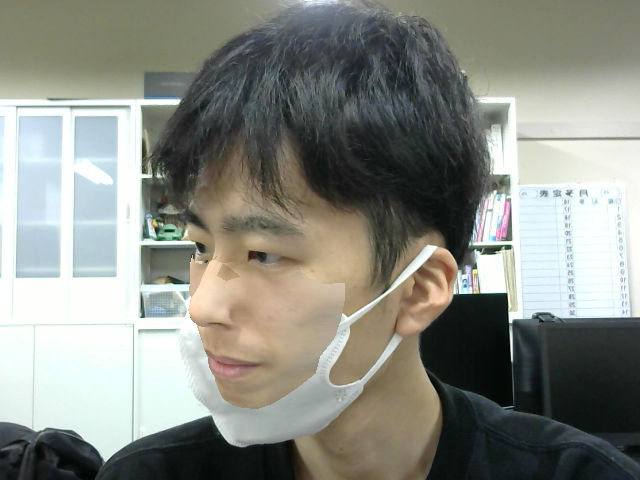
\includegraphics[keepaspectratio, scale=0.2]{figures/result/3mask/image_20231202-2.png}
      \caption{対応点:\hyperref[n441]{図\ref{n441}}の白}
    \end{minipage} &
    \begin{minipage}[t]{0.25\hsize}
      \centering
      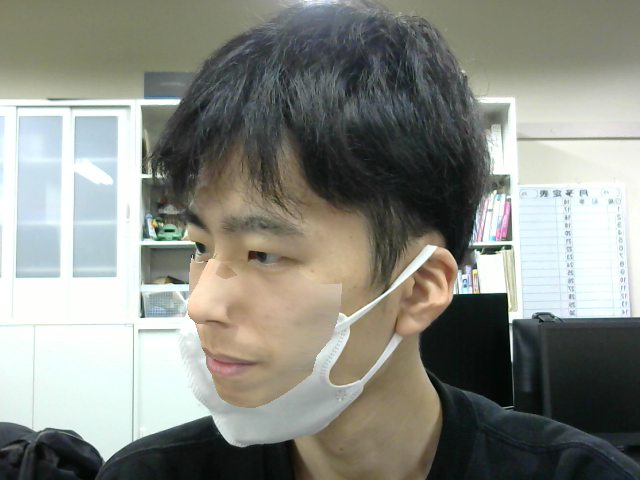
\includegraphics[keepaspectratio, scale=0.2]{figures/result/3mask/image_20231202-3.png}
      \caption{対応点:\hyperref[n441]{図\ref{n441}}の緑}
    \end{minipage}
    \begin{minipage}[t]{0.25\hsize}
      \centering
      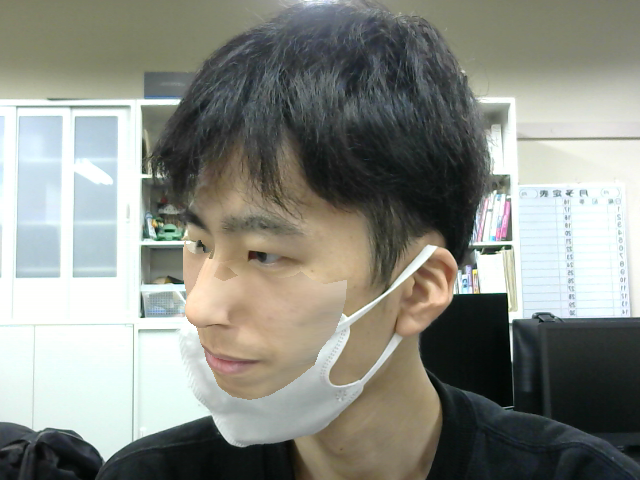
\includegraphics[keepaspectratio, scale=0.2]{figures/result/3mask/image_20231202-4.png}
      \caption{対応点:\hyperref[n442]{図\ref{n441}}の白}
    \end{minipage}
    \begin{minipage}[t]{0.25\hsize}
      \centering
      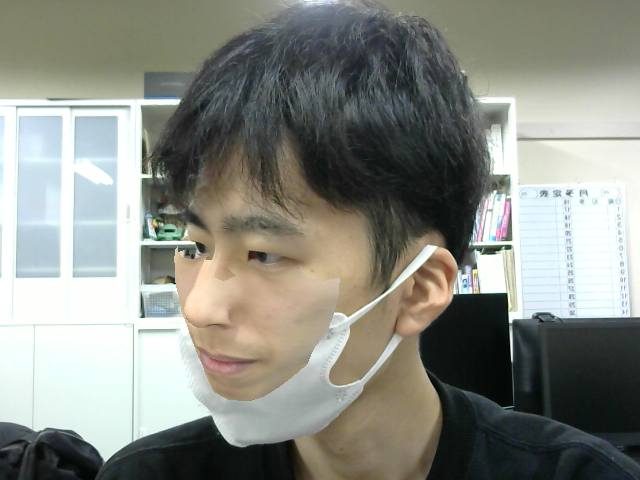
\includegraphics[keepaspectratio, scale=0.2]{figures/result/3mask/image_20231202-5.png}
      \caption{対応点:\hyperref[n442]{図\ref{n441}}の青}
    \end{minipage}
  \end{tabular}
  \caption{再現したマスク非着用画像(40°)}
  \label{n444}
\end{figure}

対応点として顔上部全体のランドマークを利用した再現画像と、顔左上部のランドマーク利用したを再現画像を比較すると、
顔左上部のランドマークを利用した画像は、三次元モデルの表示角度が画面手前側に傾いてしまっていることがわかる。
このような画像が表示された原因として、顔片側の対応点だけを用いると対応点の分布が平面に近づいてしまい、モデルの角度が
正しく計算できなかったことが考えられる。
また、マスク着用前後で安定していると判断したランドマークのみを利用した再現画像と、そうでない場合の再現画像を比較すると、
三次元モデルの大きさがやや変化したくらいで、大きく変わっていないことがわかる。

\subsection{考察}
マスク着用前後で安定していると判断したランドマークのみを利用してカメラ姿勢推定を行ったが、結果としてカメラの姿勢推定の安定性を向上させることはできなかった。
このような結果となった要因として、この一連の検証に二つの問題点があったと考える。
一つ目に、マスク着用前後で座標のずれを評価する際、完全に同位置、同姿勢で評価することができていなかったことがある。
座標のずれはかなり小さい値のため、少しでもマスク着用前後で体が動いてしまうと結果に大きく影響が出てしまう。
マスク着用前後で座標のずれの評価については複数回施行したが、ずれが小さく安定しているランドマークの選択が正しく行えていなかった可能性は否定できない。
二つ目に、カメラの姿勢推定を行う際、基本的にはより多くの対応点を用いることが推奨されていることがる。本研究では
マスク着用前後で安定しているランドマークを選択し、対応点として用いることでカメラ姿勢推定の安定性の向上を目指したが、それは必然的に全体の対応点の数が減ってしまうことを表す。
そのため安定性の向上につながらなかったのではないかと考えた。

\section{以降のスケジュール}
スケジュールについて以下にまとめる。\\
\begin{itemize}
  \item 論文に用いる資料の不足している分の撮影
  \item 対応点の変更前後でのカメラ姿勢推定結果の比較(回転行列と並進ベクトル)
  \item スライド作成
  \item 論文執筆
\end{itemize}
\end{document}
